\section{Text-2-Process}


Die Umwandlung einer informellen Beschreibung eines Geschäftsprozesses in na\-tür\-li\-cher Sprache in ein formales Prozessmodell stellt bei \ac{BPM}, wie in Kapitel 1 dargelegt, ein häufig auftretendes Problem dar. 
Der Begriff \ac{T2P} soll im Folgenden die softwaregestützte Automatisierung derartiger \ac{BPM} Umwandlungen unter Anwendung von \ac{NLP} bezeichnen.\par
Zur Realisierung von \ac{T2P} kann das aus drei sequentiellen Phasen bestehende Vorgehen zur Textanalyse nach dem State-Of-The-Art Ansatz von Friedrich gewählt werden (\cite[vgl.][4 ff.]{FRIEDRICH2}). Dieses Vorgehen macht von verschiedenen \ac{NLP} Tools Gebrauch, vor allem dem Stanford Parser, Wordnet und FrameNet (\cite[vgl.][11]{RIEFER}), welche daher im Rahmen der Arbeit vorgestellt werden.
\begin{wrapfigure}{Hr}{6cm}
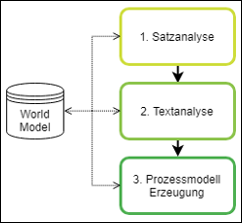
\includegraphics[width=6cm]{pictures/T2P_highlevel.png}
\caption{Vorgehen bei T2P in Anlehnung an Friedrich (eigene Darstellung)}
\label{fig:T2PHL}
\end{wrapfigure}
Abbildung \ref{fig:T2PHL} stellt das Vorgehen schematisch dar. Die einzelnen Phasen fügen dabei bezüglich des angestrebten Prozessmodels extrahierte Information inkrementell zu einer übergeordneten Datenstruktur, dem \textit{World Model}, hinzu. Parallelen zum allgemeinen Vorgehen bei NLP-ANwendungen sind deutlich erkennbar.\par
In der ersten Phase des Vorgehens werden zunächst die einzelnen Sätze im Detail analysiert. Dabei werden die grundlegenden Elemente des Prozesses ermittelt, wie etwa Akteure, Ressourcen oder Aktionen (\cite[vgl.][47 ff.]{FRIEDRICH1}). Daraufhin wird in der zweiten Phase noch einmal der Text in seiner Gesamtheit analysiert, um auch Bezüge und Beziehungen zwischen Sätzen auswerten zu können. Im Fokus stehen nun aus Prozesssicht relevante semantische Details, wie etwa die zeitliche Abfolge der in den Sätzen beschriebenen Aktionen (\cite[vgl.][66 ff.]{FRIEDRICH1}). Im dritten Schritt wird letztlich die finale Transformation in ein syntaktisch korrektes Prozessmodel vorgenommen, dies entspricht der pragmatischen Analyse. So werden etwa  eventuell entstandene Redundanzen bzw. syntaktische Unvollständigkeiten beseitigt (\cite[vgl.][90 ff.]{FRIEDRICH1}).
